The rules for the motion of billiards are straightforward. A ball moves in a straight line until it meets a boundary — where it reflects according to the law of geometric optics: the angle of incidence equals the angle of reflection. On a rectangular table, this produces familiar trajectories. Some repeat periodically, some trace diagonals, and others fill up regions with a regular structure. The behavior is fully determined by the shape of the table and the reflection rule.

When the boundary is not polygonal but curved, the situation changes. An ellipse introduces a geometric constraint absent in rectangles or circles. By definition, the sum of distances from any point on the ellipse to two fixed points, the foci, remains constant. Combined with the reflection law, this implies an optical property: any ray emanating from one focus reflects off the boundary and passes through the other. This follows from the fact that, at the point of reflection, the tangent line to the ellipse bisects the angle formed between the incoming and outgoing paths. That is, the segment from the first focus to the boundary, and then from the boundary to the second focus, meets the boundary at equal angles on either side. The configuration is symmetric, and the total path length is stationary with respect to small variations.

Most trajectories, however, do not begin at a focus. A generic path reflects from arbitrary points on the boundary. Even so, the curvature of the ellipse imposes constraints. Some paths return to their origin after a finite number of reflections; others do not. Some fill annular regions densely, never repeating. The classification of such trajectories depends on both the initial direction and the shape of the boundary.

Now consider a scenario: two nested, smooth, closed curves, an outer ellipse and an inner ellipse lying entirely within it. Imagine a polygon whose vertices lie on the outer ellipse and whose sides are tangent to the inner ellipse. This polygon represents a closed billiard path. Each segment connects two points on the outer ellipse while remaining tangent to the inner one. If such a polygon exists and closes after $n$ steps, it defines a Poncelet polygon.

The question is whether such a configuration is rare. If one closed polygon exists, does that imply anything about other starting points? Does the system admit only a single orbit, or does the existence of one periodic path imply a rule?

Poncelet’s Porism answers affirmatively. If there exists a single $n$-gon inscribed in the outer ellipse and tangent to the inner one, then for every point on the outer ellipse there exists such an $n$-gon. The ellipse is foliated by periodic trajectories of the same type. The existence of one closed polygon implies the existence of an infinite family, each differing only by a rotation of the starting point.

\begin{center}
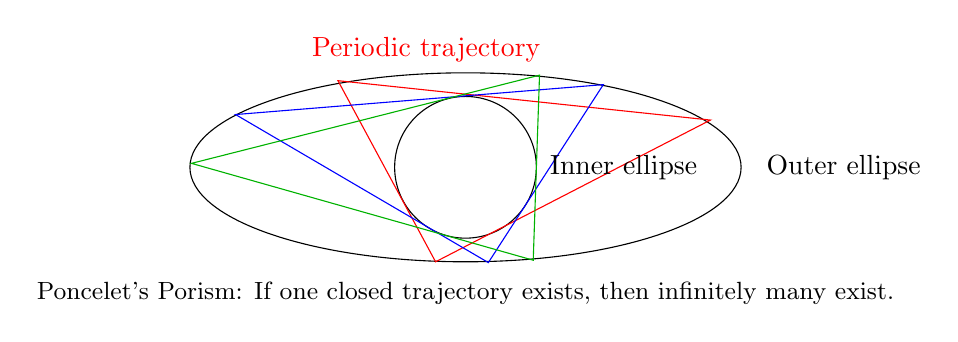
\begin{tikzpicture}[scale=1]
    % Define the ellipse and circle
    \draw (0,0) ellipse (3.5cm and 1.2cm);
    \draw (0,0) circle (0.9cm);
    
    % First triangle (red)
    \draw[red] (-1.62, 1.1) -- (-0.38, -1.2) -- (3.11, 0.6) -- cycle;
    
    % Second triangle (blue)
    \draw[blue] (-2.92, 0.67) -- (0.29, -1.21) -- (1.75, 1.05) -- cycle;
    
    % Third triangle (green)
    \draw[green!70!black] (-3.48, 0.05) -- (0.86, -1.18) -- (0.94, 1.17) -- cycle;
    
    % Annotations
    \node[right] at (3.7, 0) {Outer ellipse};
    \node[right] at (0.95, 0) {Inner ellipse};
    \node[red] at (-0.5, 1.5) {Periodic trajectory};
    \node[font=\small] at (0, -1.6) {Poncelet's Porism: If one closed trajectory exists, then infinitely many exist.};
\end{tikzpicture}
\end{center}

The geometric construction of Poncelet polygons can be reinterpreted as a dynamical process. Fix two nested ellipses. Choose a point on the outer ellipse and draw a line tangent to the inner ellipse, continuing the segment until it intersects the outer ellipse again. Repeat this procedure: from each new intersection, draw the unique line tangent to the inner ellipse and find its next point of contact with the outer ellipse. The result is a discrete sequence of points on the outer ellipse, each determined from its predecessor by a geometric rule. This iteration defines a map from the outer ellipse to itself.

This map — commonly referred to as the Poncelet map — sends a point on the outer ellipse to the next vertex of the corresponding Poncelet polygon. It depends only on the two ellipses and the tangency construction. The rule is deterministic: one point determines the next, and the process can continue indefinitely.

The Poncelet map preserves a finite, non-atomic measure on the outer ellipse. This means there exists a way to assign consistent arc-length values to intervals such that the total measure remains unchanged under iteration. The map may distort the shape of regions, but it does not compress or expand their measure. This symmetry is specific to the geometry of the construction and is not typical for transformations on curves.

This property allows for a complete classification. Every orientation-preserving, measure-preserving transformation of a circle is either conjugate to a rigid rotation or exhibits more complicated behavior, such as wandering intervals. The Poncelet map falls into the first case — there exists a homeomorphism, a continuous, invertible change of coordinates, that maps the ellipse to a circle and transforms the Poncelet map into a pure rotation by a fixed angle.

This angle, defined modulo $2\pi$, is the rotation number. It measures the average angular advance per iteration, and its arithmetic character determines the long-term behavior of orbits. If the rotation number is a rational multiple of $2\pi$, say $2\pi p/q$, then every point on the circle returns to its starting position after $q$ steps. In the original geometry, this corresponds to a Poncelet polygon with $q$ sides. Every orbit closes, and the ellipse is covered by congruent, rotated versions of the same path. If the rotation number is irrational, no orbit closes. Each point traces a dense, non-repeating sequence along the ellipse.

(Side note: A \emph{porism} asserts that if one configuration satisfying given conditions exists, then a whole family exists as well. Theorems give a single existence; a porism promotes it to a family parameterized by starting point. Which reminds me of the joke by mathematician Jerry Bona, in which he described the equivalence of the Axiom of Choice, Zorn’s Lemma, and the Well-Ordering Theorem as follows: \textbf{"The Axiom of Choice is obviously true, the Well-Ordering Theorem is obviously false, and Zorn’s Lemma — who can tell?"} These statements are mathematically equivalent, yet their perceived plausibility varies widely.)

Poncelet originally proved his porism in 1822 using projective geometry and the theory of conics. Later approaches employed algebraic geometry, treating the problem as a question about curves in complex projective space. The configuration of two nested conics defines an elliptic curve, and the closure condition corresponds to torsion points on this curve. These methods, while powerful, require sophisticated machinery from algebraic geometry and complex analysis.

The dynamical systems approach sidesteps this complexity entirely. Rather than working with elliptic curves or projective transformations, it recognizes the Poncelet map as a measure-preserving transformation conjugate to a rotation. The geometric fact — that this particular map preserves measure — replaces pages of algebraic manipulation. Once established, the porism follows immediately from elementary properties of circle rotations.

This same framework appears in problems involving the distribution of leading digits in exponential sequences. The following analysis concerns the frequency of initial digits in powers of integers, governed by irrational rotations on the unit interval.

Consider the powers of 2: $2^1 = 2$, $2^5 = 32$, $2^{10} = 1024$, $2^{53} = 9{\,}007{\,}199{\,}254{\,}740{\,}992$. Some begin with 1, others with 3, 9, etc. The digits appear irregularly, but over time, a pattern emerges. The frequency of each digit stabilizes and matches a specific distribution.

The explanation is logarithmic. Write $2^n = 10^{n \log_{10} 2}$. The number of digits in $2^n$ grows roughly linearly in $n$, and its leading digit depends only on the decimal part of $n \log_{10} 2$. As $n$ increases, the sequence $\{ n \log_{10} 2 \}$ fills the interval $[0,1)$ evenly, because $\log_{10} 2$ is irrational. This means that $2^n$ is equally likely to appear in any logarithmic subinterval of a given order of magnitude.

A number begins with digit $d$ if its logarithm lies between $\log_{10} d$ and $\log_{10}(d+1)$. So the proportion of terms $2^n$ that begin with digit $d$ approaches
\[
\log_{10}\left(1 + \frac{1}{d}\right).
\]
This is Benford’s Law. It predicts that 1 appears as the leading digit about 30\% of the time, while 9 appears less than 5\% of the time. The same reasoning applies to any base-$b$ sequence where $\log_{10} b$ is irrational. The decimal parts of $n \log_{10} b$ become evenly spread, and the digit frequencies converge to the same logarithmic formula.

Benford's Law extends far beyond powers of integers. Real-world datasets that span multiple orders of magnitude — river lengths, city populations, physical constants, file sizes, mountain heights — often follow the same logarithmic distribution. The key requirement is that the data range widely without artificial constraints or preferred scales.

When values are distributed across many orders of magnitude, they tend to be spread evenly on a logarithmic scale rather than a linear one. This occurs naturally when data arise from multiplicative processes or when no particular scale is privileged. In such cases, the probability of a value falling into the interval that starts with digit $d$ is proportional to the logarithmic length of that interval: $\log_{10}(1 + 1/d)$. This geometric fact, combined with scale invariance, produces Benford's distribution without requiring randomness or special assumptions. This property makes Benford's Law useful for fraud detection, where artificial datasets often deviate from the expected pattern.

Benford’s Law does not apply universally. It fails when numbers are tightly clustered, rounded, or constrained by conventions, such as ID numbers, product prices, or phone records. But when applicable, it can serve as a diagnostic tool. Large deviations from the expected digit frequencies may indicate fabricated or manipulated data.

Forensic accountants have used Benford's Law to uncover anomalies in financial statements, including during the Enron scandal. Tax authorities apply it to detect suspicious filings. In the 2009 Iranian presidential election, statistical tests based on Benford’s Law identified irregularities in reported vote counts. In each case, observed digit distributions diverged significantly from the logarithmic baseline, suggesting artificial data generation.

This formulation, noted by Gelfand, is identical to the classification of the Poncelet map. In both cases, a rotation acts on a compact one-dimensional space, and the long-term behavior of orbits (whether periodic or equidistributed) depends only on the rationality of a single parameter. For powers of $b$, this parameter is $\log_{10} b$; for the Poncelet construction, it is the angular step induced by tangency. 

\begin{commentary}[Commentary: On Invariant Measures and Unexpected Turns]
I began to love mathematics during my undergraduate studies, particularly through a set theory course taught by Professor Amos Nevo. The material was foundational, focusing on logic, sets, and proofs. Nevo consistently highlighted how abstract structures recur across fields, enhancing its significance. Even when teaching introductory content, he pointed toward broader connections: between algebraic symmetries, analysis, and geometry.

Later, in a seminar on dynamical systems (we were a group of students who tried to enroll in any course Amos offered), he asked me to present a proof of Poncelet’s Porism. I began working through the classical approach: projective geometry, dual conics, and elliptic curves. After several weeks of effort, I came to him with the outline. He laughed and said that wasn’t the proof he had in mind.

Instead, he pointed me to a short argument we had already studied in class, one based on the existence of an invariant measure. From that, topological conjugacy implies that the Poncelet map behaves like a rigid rotation. Rational rotation number implies periodicity. The porism drops out almost immediately.

The Poncelet map is a beautiful object and exemplifies how abstract tools from dynamical systems, such as invariant measures and topological conjugacy, can be seen doing the heavy lifting on a classical geometry problem. It was also one of the best seminars I ever took for accelerating mathematical maturity.
\end{commentary}

\vspace{2em}
\begin{center}
    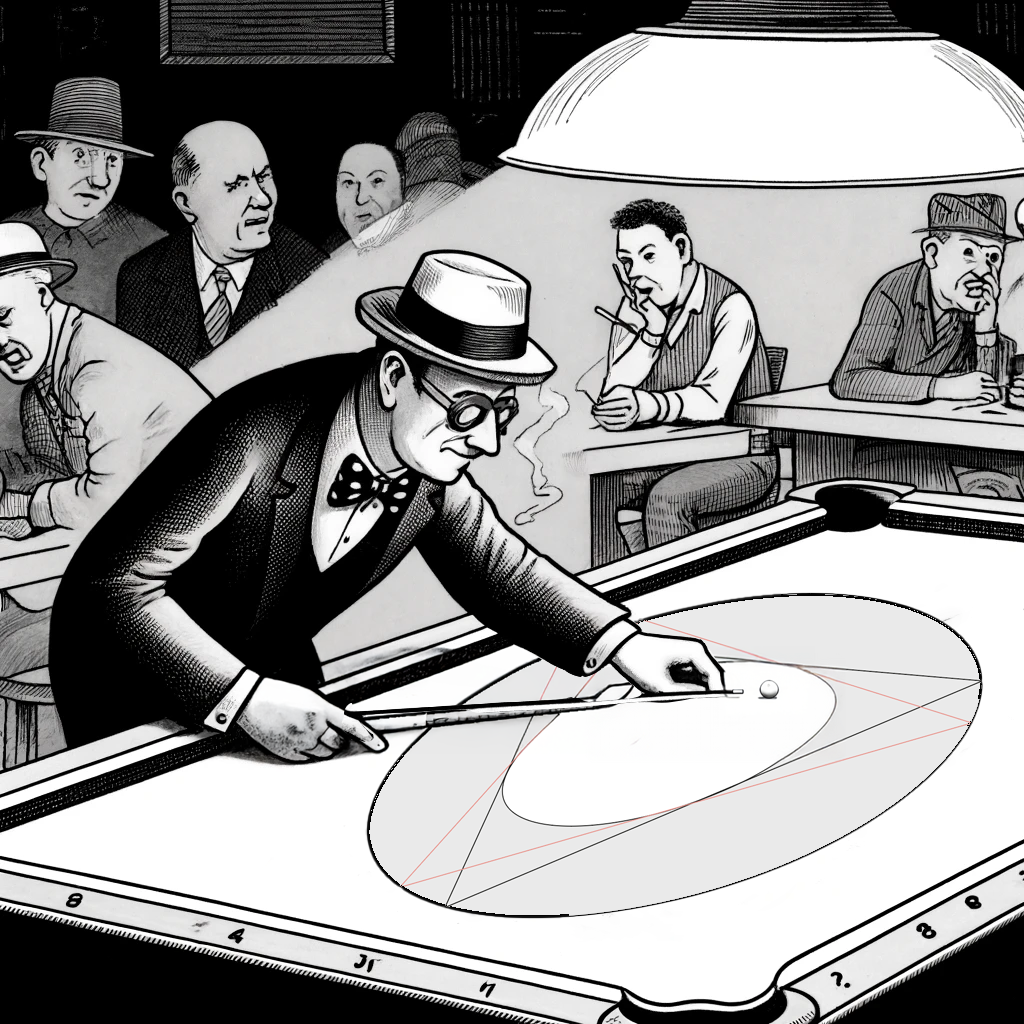
\includegraphics[height=10\baselineskip]{07_BilliardsConicsPorism/BILLIARDS.png}\\
    {\small\textit{Mike's understanding of Snell's law made him unbeatable,\\ but considerably slowed down the game}}
\end{center}